\chapter{Work Harder On Yourself Not On Your Job}

This chapter comes from a Jim Rohn lecture preserved in a curated playlist from LazyingArt LLC. No validated board screenshots survive for this lecture, so we let the transcript carry the mathematical structure and write down only those relations that the speaker actually motivates: first the shift from blame to response, then the shift from response to self-change, then the shift from money to value, and finally the return from economics to the larger labor of working on oneself.

\section{From Blame to Responsibility}

Rohn begins by telling us that personal development was hard for him because it required surrendering a very comfortable explanatory system. He could blame government, relatives, company policy, unions, wage scale, the economy, interest rates, prices, and circumstances. The lecture does not open with a theorem but with the emotional cost of abandoning the wrong variable.

His mentor then introduces the first sharp principle. What happens does not determine the major part of the future. What matters is what we do about what happens. The logic is simple and powerful: if what happens happens to all of us, then mere event cannot be the whole explanation of divergence.

\subsection{Question \& Answer}

\paragraph{Question.} What determines the major part of the future?

\paragraph{Answer.} Not bare occurrence, but response. The speaker's first move is to shift the active variable from what happens to what we do about it.

We can write the cleaned relation as
\begin{equation}
\text{Major part of the future} \Longleftarrow \text{what we do about what happens}.
\end{equation}

And the corresponding negation is
\begin{equation}
\text{What happens} \not\Longrightarrow \text{major part of the future}.
\end{equation}

The chapter should keep the order here. First the confession, then the mentor's correction. Otherwise the formula will sound too easy.

\section{The Ninety-Day Experiment}

Once the response variable has been isolated, the lecture immediately asks how we test it. The answer is not metaphysical. Do something different over the next ninety days than over the last ninety days. Read different books. Adopt new health disciplines. Alter conduct in family life. The examples are small on purpose. Rohn wants the audience to see that the mechanism begins locally.

The important constraint is that circumstances remain substantially the same. We cannot, in his phrasing, change the circumstances. We can change ourselves. We can change what we do. A compact reconstruction is
\begin{align}
C_{1} &= C_{0},\\
A_{1} &\neq A_{0},\\
R_{1} &\neq R_{0},
\end{align}
where \(C\) denotes circumstances, \(A\) action, and \(R\) result. This is not his notation, but it is the cleanest way to preserve his operational claim.

So the lecture's first update rule is already in place: same outer field, altered conduct, altered result. That naturally prepares the next and harder claim, namely that what we presently possess is not accidental with respect to the self that has produced it.

\section{What We Have, What We Have Become}

Rohn's next secret is more severe. What we have at the moment, he says, we have attracted by the person we have become. This is where the lecture leaves ordinary encouragement and becomes explanatory. The present state is not merely unfortunate; it is fitted to the present self.

\begin{equation}
\text{What you have now} \Longleftarrow \text{the person you've become}.
\end{equation}

He then forces the rule onto biography. Pennies in pocket, nothing in the bank, creditors calling, promises behind. The speech slows down here because the principle must first be made painful before it can become useful. Only then does he ask the question that the chapter should preserve in its own right.

\subsection{Question \& Answer}

\paragraph{Question.} How can I change all that?

\paragraph{Answer.} By changing the person who has been attracting the present condition. The corrective variable is inside, not outside.

This gives the lecture its governing formula:
\begin{equation}
\text{Everything changes for you} \Longleftarrow \text{You change}.
\end{equation}

Rohn immediately expands the same thought in two further steps. First, we do not have to change what is outside. Second, to have more we must become more:
\begin{align}
\text{Change what is inside} &\Longrightarrow \text{change what is outside for you},\\
\text{Have More} &\Longleftarrow \text{Become More}.
\end{align}

The little paired imperatives that follow are not detachable aphorisms. They are short forms of the same rule:
\begin{align}
\text{Wish you were better} &> \text{wish it were easier},\\
\text{Wish for more skills} &> \text{wish for fewer problems}.
\end{align}

\section{Money as the First Diagnostic}

Only after establishing the self-change formulas does Rohn pivot to economics. He says that in helping children understand personal development he always starts with money. The reason is not that money is the only value. The reason is that money is countable.

\begin{equation}
\text{Money}=\text{a first countable diagnostic of personal development}.
\end{equation}

This is a pedagogical move, and the chapter should preserve it as such. We are not leaving the first half of the lecture behind. We are testing it in a domain where the consequences are numerically legible. Hence the next step: we get paid for bringing value to the marketplace.

\section{Value, Time, and Pay}

The economic spine of the lecture is now introduced very carefully. We get paid for bringing value to the marketplace. Marketplace is then glossed as reality. The extra word matters: it tells us that the lecture is not talking about moral approval, only about the environment that prices contribution.

\begin{align}
\text{We get paid for bringing value to the marketplace},\\
\text{Marketplace}=\text{Reality}.
\end{align}

Time enters immediately after, but only as a medium. It takes time to bring value to the marketplace, but we do not get paid for time. This is the first explicitly corrective moment in the economic argument.

\subsection{Question \& Answer}

\paragraph{Question.} Do we get paid for time or for value?

\paragraph{Answer.} Time is necessary, but value is what is bought. The lecture rejects the common speech according to which one is simply paid so much ``for an hour.''

In cleaned form:
\begin{align}
\text{Time is required to bring value to the marketplace},\\
\text{Pay} \neq \text{Time alone},\\
\text{You get paid for the value you put in the time}.
\end{align}

A cautious symbolic compression, useful for note-writing but not spoken in the lecture, is
\begin{equation}
P \propto V \qquad (T \text{ fixed}),
\end{equation}
where \(P\) is pay, \(V\) value, and \(T\) time. The point is modest: once time is held fixed, value is the variable that can move the result.

This makes possible the lecture's first clean quantitative puzzle.

\section{More Money in the Same Time}

Rohn now asks whether it is possible to become twice as valuable and make twice as much money in the same time. This is the moment when the lecture becomes most nearly mathematical in the narrow sense, because the variable held fixed is time.

\subsection{Question \& Answer}

\paragraph{Question.} Is it possible to make more money in the same time?

\paragraph{Answer.} Yes. If the same time contains more value, then the same time can yield more money.

A clean worked version is
\begin{align}
T_{1} &= T_{0},\\
V_{1} &= 2V_{0},\\
P_{1} &= 2P_{0}.
\end{align}

The lecture does not insist on this notation, but it does insist on the logic. Hence the summary line:
\begin{equation}
\text{Earn more money in the same time} \Longleftarrow \text{Become more valuable}.
\end{equation}

This conclusion is immediately translated into image. America is not a bed. It is a ladder.

\section{The Ladder, Reality, and Opportunity}

The ladder image lets Rohn move from a proportionality statement to a picture of ascent. The ladder starts down near \(\$4\) an hour. The debate over whether the starting place should be five dollars is answered by shifting the real question: are we planning to remain at the bottom, or to climb?

\begin{equation}
\text{America}=\text{a ladder to climb}.
\end{equation}

\begin{equation}
\text{America} \neq \text{a bed}.
\end{equation}

\begin{figure}[h]
\centering
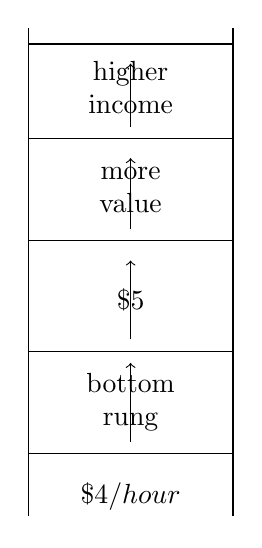
\begin{tikzpicture}
\draw (-1.3,0) -- (-1.3,6.2);
\draw (1.3,0) -- (1.3,6.2);
\draw (-1.3,0.8) -- (1.3,0.8);
\draw (-1.3,2.1) -- (1.3,2.1);
\draw (-1.3,3.5) -- (1.3,3.5);
\draw (-1.3,4.8) -- (1.3,4.8);
\draw (-1.3,6.0) -- (1.3,6.0);
\node at (0,0.25) {\(\$4/\text{hour}\)};
\node[align=center] at (0,1.45) {bottom\\rung};
\node at (0,2.75) {\(\$5\)};
\node[align=center] at (0,4.15) {more\\value};
\node[align=center] at (0,5.45) {higher\\income};
\draw[->] (0,0.95) -- (0,1.95);
\draw[->] (0,2.25) -- (0,3.25);
\draw[->] (0,3.65) -- (0,4.55);
\draw[->] (0,4.95) -- (0,5.75);
\end{tikzpicture}
\caption{Transcript-derived ladder reconstruction. No validated board frame survives for this lecture, so the figure is drawn directly from the spoken argument.}
\end{figure}

The ladder by itself is not enough. Rohn then introduces a crucial distinction. One may be valuable to the human family, to the church, to the community, and still not be very valuable to the marketplace. The lecture needs this distinction because otherwise the wage discussion would collapse into a claim about total human worth, which it is not.

\begin{align}
\text{Low marketplace value} &\Longrightarrow \text{Low marketplace pay},\\
\text{Demand} &\not\Longrightarrow \text{Riches},\\
\text{Climb} &> \text{wait for a raise}.
\end{align}

\subsection{Question \& Answer}

\paragraph{Question.} How do we get more money?

\paragraph{Answer.} Not by demand, and not by passive waiting, but by becoming more valuable.

The lecture then proves its own claim by anecdote. A company calls with a project worth millions because it is expanding internationally and needs help. The garbled portions of the transcript should not be forced into detail; the stable point is the causal one:
\begin{equation}
\text{Telephone call worth millions} \Longleftarrow \text{I had become valuable}.
\end{equation}

This anecdote allows Rohn to restate the first half of the lecture in economic language: if he later attracted a call worth millions, whereas earlier he had pennies in his pocket, then the person in between must have changed.

\section{Work Harder on Yourself}

The closing maxim gathers the chapter into a final pair of relations:
\begin{align}
\text{Work hard on your job} &\Longrightarrow \text{Make a living},\\
\text{Work hard on yourself} &\Longrightarrow \text{Make a fortune}.
\end{align}

The lecture immediately protects this from sounding purely monetary. Rohn says that he was already a hard worker when he was poor; the problem was not the absence of effort but the location of effort. He was working hard on his job, not on himself. That distinction then expands into a whole program: work on skills, graces, philosophy, attitude, personality, language, communication, and the rest of one's abilities.

The agricultural analogies at the end carry the same message in another register. Do not try to change the seed, the soil, the sunshine, the rain, the seasons. Work on the inside. That is why the final recurrence of the chapter's opening law is not redundant. It is the lecture returning to its own governing variable.

\section{Summary}

This lecture begins with the surrender of blame and ends with the labor of self-development. Between those two points it builds a small but coherent mathematics. First, what happens is distinguished from what we do about it. Second, present condition is linked to the person we have become. Third, change is relocated from the outside to the inside. Fourth, money is introduced as a countable diagnostic. Fifth, pay is tied to value rather than to time alone. Sixth, the ladder image translates the same principle into public economic life. And finally, the whole argument is brought back to self-work.

The shortest faithful summary is still the strongest one:
\begin{equation}
\text{Everything changes for you} \Longleftarrow \text{You change}.
\end{equation}

And the most practical companion to it is this:
\begin{equation}
\text{Work on yourself} \Longrightarrow \text{Become more valuable to the marketplace}.
\end{equation}

That is the lecture's full circle: change response, change self, change value, change result.